\documentclass[letterpaper, 10 pt, conference]{ieeeconf}  % Comment this line out if you need a4paper

\IEEEoverridecommandlockouts
\overrideIEEEmargins

\title{\LARGE \bf
Provably correct sensor-driven path-following for unicycles using monotonic score functions
}


\author{Benton Clark$^{1}$, Varun Hariprasad$^{2}$, and Hasan A. Poonawala$^{1}$%
\thanks{*This work was not supported by any organization}%
\thanks{$^{1}$Benton Clark and Hasan A. Poonawala are with Faculty of Mechanical and Aerospace Engineering,
        University of Kentucky, Lexington, KY 40506, United States
        {\tt\small \{benton.clark,hasan.poonawala\}@uky.edu}}%
\thanks{$^{2}$ Varun Hariprasad is a student at Paul Laurence Dunbar High School,
1600 Man o' War Boulevard, Lexington, KY 40513, United States
{\tt\small varunhpr5@gmail.com}}%
}

\usepackage[utf8]{inputenc}
\usepackage{subcaption}
\usepackage{graphicx}
\usepackage{amsmath}
\usepackage{amssymb}
\usepackage{todonotes}
\usepackage{leftidx}
\usepackage{tikz}
\usepackage{pgfplots}
\usetikzlibrary{arrows,decorations.pathmorphing,positioning,fit,trees,shapes,shadows,automata,calc,intersections,decorations.markings,pgfplots.fillbetween,patterns} 

\setlength{\marginparwidth}{2cm}
\usepackage[normalem]{ulem}
\newcommand{\hlc}[1]{\bgroup\markoverwith
  {\textcolor{#1}{\rule[-1ex]{2pt}{2.5ex}}}\ULon}
\newcommand{\hlctodo}[2]{\todo[color=#1]{#2}\bgroup\markoverwith
  {\textcolor{#1}{\rule[-.5ex]{2pt}{2.5ex}}}\ULon }
\usepackage{hyperref}
\hypersetup{colorlinks=true,     
linkcolor=blue,          % color of internal links
        citecolor=blue,        % color of links to bibliography
          filecolor=magenta,      % color of file links
           urlcolor=magenta           % color of external links
}


% Custom commands for mobile robot kinematics
\newcommand{\phit}{\phi(t)}
\newcommand{\ppath}{\mathcal{P}}
\newcommand{\dset}{\mathcal{D}}


% Commands for StBSF and SeBSF
\newcommand{\stbsf}{F}
\newcommand{\sebsf}{\Tilde{F}}


% Custom commands for LS analysis
\newcommand{\Qone}{\overline{Q}_1}
\newcommand{\Qtwo}{\overline{Q}_2}
\newcommand{\Qthr}{\overline{Q}_3}
\newcommand{\Qfor}{\overline{Q}_4}
\newcommand{\Qoneic}{\Qone^L}
\newcommand{\Qthric}{\Qthr^L}
\newcommand{\Xo}{X_0}
\newcommand{\tlb}{\underline{\theta}}
\newcommand{\tub}{\overline{\theta}}
\newcommand{\dlb}{\underline{d}}
\newcommand{\dub}{\overline{d}}

% Commands for d-\theta figure
\newcommand{\pathfunc}{\gamma}
\newcommand{\switchsurf}{\alpha}
\newcommand{\deviation}{d}
\newcommand{\localangle}{\theta}
\newcommand{\locstate}{\state}
\newcommand{\exaenvir}{\rho}

% Custom commands
\newcommand{\Ftx}{F(\theta,x)}
\newcommand{\Ftd}{F(\theta,d)}
\newcommand{\gtx}{g(\theta,x)}
\newcommand{\R}{\mathbb{R}}
\newcommand{\N}{\mathbb{N}}
\newcommand{\oF}{\overline{F}}
\newcommand{\uF}{\underline{F}}
\newcommand{\oFd}{\overline{F}_\delta}
\newcommand{\pd}[2]{\frac{\partial #1}{\partial #2}}
\newcommand{\bmat}[1]{\begin{bmatrix}#1\end{bmatrix}}
\newcommand{\bigpar}[1]{\left( #1 \right)}
\newcommand{\sign}[1]{\mathrm{sign} #1 }
% Commands: Frames and Kinematics
\newcommand{\Frame}{\mathcal{F}}
\newcommand{\origin}{\mathcal{O}}
\newcommand{\ihat}{\hat{i}}
\newcommand{\jhat}{\hat{j}}
\newcommand{\khat}{\hat{k}}
\newcommand{\vd}{\vec{d}}
\newcommand{\vt}{\vec{\theta}}
\newcommand{\vx}{\vec{x}}
\newcommand{\vc}{\vec{c}}
\newcommand{\vxe}{\vec{x}_e}
\newcommand{\vxz}{\vec{x}_0}
\newcommand{\vv}{\vec{v}}
\newcommand{\vy}{\vec{y}}
\newcommand{\vw}{\vec{\omega}}
\newcommand{\vr}{\vec{r}}
\newcommand{\vrp}{\vec{r}\;'}
\newcommand{\ve}{\vec{e}}
\newcommand{\vq}{\vec{q}}
\newcommand{\dvr}{\dot \vr}
\newcommand{\qdes}{\vec q_{\text{des}}}
\newcommand{\Qss}{\mathcal{Q}}
\newcommand{\fproj}{f_\text{proj}}

% Commands: LS / LAS Analysis
\newcommand{\Qonenot}{Q_{\star 0}^1}
\newcommand{\Qthrnot}{Q_{\star 0}^3}
\newcommand{\XLp}{X_{L}^+}
\newcommand{\XLm}{X_{L}^-}
\newcommand{\XLo}{X_{L^0}}
\newcommand{\dbound}{d_\star}
\newcommand{\tbound}{\theta_\star}
\newcommand{\vctrl}{\beta e^{-\alpha \stbsf^2}}
\newcommand{\vctrlsebsf}{\beta e^{-\alpha \sebsf^2}}
\newcommand{\invf}[1]{{#1}^{-1}}
% Differentiate w.r.t. frame input
\newcommand{\difff}[2]{\leftidx{^{#1}}{\frac{d #2}{dt}}}
% Differentiate w.r.t. the 0 frame
\newcommand{\difffz}[1]{\difff{0}{#1}}
\DeclareMathOperator{\sgn}{sgn}

\newtheorem{lemma}{Lemma}
\newtheorem{fact}{Fact}
\newtheorem{theorem}{Theorem}
\newtheorem{remark}{Remark}
\newtheorem{definition}{Definition}

\begin{document}

\maketitle
\thispagestyle{empty}
\pagestyle{empty}
\begin{abstract}
This paper develops a provably stable sensor-driven controller for path-following applications of robots with unicycle kinematics, one specific class of which is the wheeled mobile robot (WMR). %
The sensor measurement is converted to a scalar value (the score) through some mapping (the score function); the latter may be designed or learned. 
The score is then mapped to forward and angular velocities using a simple rule with three parameters. 
The key contribution is that the correctness of this controller only relies on the score function satisfying monotonicity conditions with respect to the underlying state -- local path coordinates --  instead of achieving specific values at all states. %
The monotonicity conditions may be checked online by moving the WMR, without state estimation, or offline using a generative model of measurements such as in a simulator.
Our approach provides both the practicality of a purely measurement-based control and the correctness of state-based guarantees. 
We demonstrate the effectiveness of this path-following approach on both a simulated and a physical WMR that use a learned score function derived from a binary classifier trained on real depth images. 
\end{abstract}





\section{Introduction}
\label{sec:intro}
Mobile robot navigation is a long-standing topic of research and development in robotics. %
A primary navigation problem is to follow a path~\cite{micaelli1993trajectory,wit1993nonlinear,rio_pathfollowing_1999}, such as defined by lanes on a highway or the walls of a hallway. %
The path is typically assumed free of obstacles, but straying too far from the path may cause collisions. %
Therefore, we would like the robot to stay within some distance from the path due to the possible collisions with objects. 

Traditional approaches to the path-following problem look at designing controllers with provable guarantees of the system stability, assuming direct state measurements are available for feedback~\cite{wit1993nonlinear}. %
The state is typically the distance to a point on the path and the relative heading to the path. %
Measuring these quantities in unstructured environments is difficult or impossible, which limits deployment of mobile robots in such settings. 

In order to avoid direct state measurement, several groups have focused on learning direct sensor-to-actuator feedback controllers~\cite{levine2016end,giusti2015machine}. 
Most of these methods use deep neural networks~\cite{Goodfellow2016DLbook} to map high-dimensional measurements from on-board sensors (e.g.\ optical camera, LiDAR) to control input values, without intermediate state estimation. %
The drawback of these approaches is that they do not provide guarantees on the system stability or convergence to the path for the resulting closed-loop system. %
These methods also require significant data and computational resources~\cite{levine2016end}. 

This lack of guarantees for learned controllers has prompted new controller synthesis and verification methods~\cite{chang2019neural,reedverified,rpm,poonawala2021training}. %
In principle, the methods could enable provably correct sensor-driven control. %
However, they suffer from two drawbacks related to path-following, especially in unstructured environments.
First, the guarantees rely on prior knowledge of a measurement model that predicts measurements that would be obtained around the path. 
This model may be difficult to obtain, and the guarantees are brittle to variation in the real mapping from local path coordinates to sensor measurements that will occur when deployed in changing environments. %
Second, the synthesis and verification of these methods is often computationally expensive, preventing a possible solution where new verified controllers are computed in response to changing environments.

The method in~\cite{poonawala2021training} attempts to overcome the issue of changing environments by using discrete control inputs predicted by a classifier. They argue that the changing measurement model  is equivalent to a variable switching surface in the state space. Using differential inclusion models, they guarantee that deviation from the path are bounded despite uncertainty in the measurement model. This robustness is obtained at the expense of producing a discontinuous switching controller, which is undesirable for real hardware systems. Additionally, the human designer must still choose the number and value of the discrete inputs. 

Ideally, we wish to obtain a sensor-driven path-following controller with guaranteed behavior that does not rely on online state estimation or offline measurement prediction. %

\paragraph*{Contributions} 
This paper proposes a sensor-driven path-following control approach where a high-dimensional sensor measurement is mapped to a scalar value which is in turn mapped to forward and angular velocities of a robot with unicycle kinematics. 
The main contribution is to show that this mapping -- called the Sensor-based Score Function -- from sensor to scalar value must satisfy conditions that do not rely on knowing the measurement obtained in a state \emph{a priori}.  
Additionally, the mapping from scalar value to control inputs is simple with only three parameters that we describe how to choose.
A consequence of this approach is that a measurement model is not necessary when designing the controller, and the guarantees are robust to changes in the measurement model during deployment.
The score function thus enables a connection between pure measurement-based control and rigorous state-based analysis.
We provide results of simulated and physical path-following experiments to demonstrate the benefits of this approach.


\newcommand{\curv}{\rho}
\section{Path-Following Problem}
\label{sec:kinematics}
We consider mobile robots with unicycle kinematics~\cite{malu_kinematics_2014}. Given a one-dimensional curve $\ppath$ in the plane, we can express the kinematics in a local state-space representation known as the ``orthogonal projection''~\cite[p.132]{wit1993nonlinear} of the robot's centroid $P$ about a path $\ppath$. 
The system dynamics consist of the following equations:
\begin{align*}
     \dot s &= v\cos\theta/(1-\curv(s)d), \\ % \label{eq:sdot}
     \dot d &= v\sin\theta, \text{ and}\\ %\label{eq:ddot}
     \dot \theta &= \omega - v\cos(\theta)\curv(s)/(1-\curv(s)d), %\label{eq:tdot-full} \
\end{align*}
where $s$ is the arc length along the curve $\ppath$, 
$\curv(s)$ is the path's curvature at the distance $s$, 
$d$ is the signed distance of the point $P$ from the path, 
$\theta$ is the difference between the heading direction of the WMR and the tangent to the path, 
$v$ is the forward velocity control input, and 
$\omega$ is the angular velocity control input.
The state space values are derived from a Frenet-Serret frame attached along the path $\ppath$ whose normal coincides with the point $P$.
Figure~\ref{fig:ddwmr} provides an illustration of this parameterization.

The \textbf{path-following problem} is to ensure that $d(t) \to 0$ as $t \to \infty$ and that $\dot s(t) > 0$ for all time. 
Note that for paths with time-varying curvature, convergence to the path is impossible without feed-forward control of the path. 
Therefore, our analysis will focus on the case of straight paths.
The convergence guarantees we obtain for the straight-line paths imply bounded deviations for the curved-path case, as argued in~\cite{reedverified}. %

%%%%%%%%%%% Differential drive
\newcommand{\ddtikz}[3]{
\begin{scope}[xshift=#1cm,yshift=#2cm,rotate=#3,scale = 1.3]
\draw[thick,rounded corners=0.04cm] (-0.3,-0.3) rectangle (0.3,0.3);
\draw[thick,rounded corners=0.04cm,pattern=vertical lines] (-0.5,0.35) rectangle (0.5,0.5);
\draw[thick,rounded corners=0.04cm,pattern=vertical lines] (-0.5,-0.5) rectangle (0.5,-0.35);
\draw[thick] (0.15,0) +(0.25,-0.15) -- +(0.15,-0.1) -- +(0.15,0.1) -- +(0.25,0.15) -- cycle;
\draw[fill = blue,thick] (0,0) circle (0.05) node[left]{P};
% \draw[fill = red,thick] (0.35,0) circle (0.05);
% \draw[fill = green!70!black,thick] (0,0.425) circle (0.05);
% \draw[fill = orange,thick] (0,-0.425) circle (0.05);

\end{scope}
}

\begin{figure}[tb]
\centering
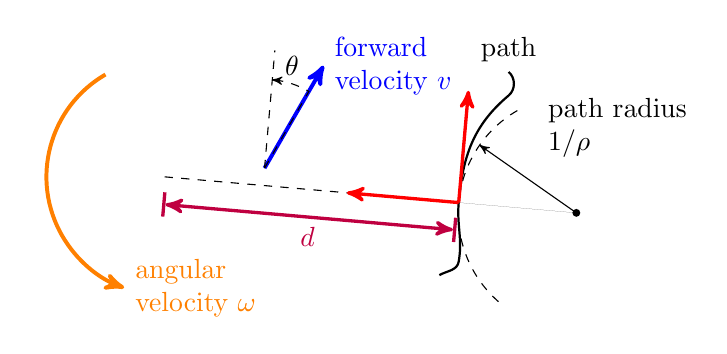
\begin{tikzpicture}[scale=1.0,>=stealth']
\coordinate (orig) at (0,0);
\def\xaxissize{1.5}
\def\yaxissize{1.5}
\def\robotrotate{60}
\def\axisangle{-65}
\ddtikz{0}{0}{60}
% forward velocity:
\coordinate (fvelbase) at ($(orig)+(10+\robotrotate+\axisangle:0.85*\xaxissize)$);
\draw[->,color=blue,line width = 0.5mm] (fvelbase) -- ($(fvelbase)+(0+\robotrotate:1.0*\xaxissize)$) node[right,blue,text width = 2cm] {forward \\ velocity $v$};
\draw[->,dashed] (fvelbase) -- ($(fvelbase)+(0+\robotrotate:0.75*\xaxissize)$) arc (0+\robotrotate:\robotrotate+\axisangle+90:0.75*\xaxissize);
\node[->,dashed] at ($(fvelbase)+(0+\robotrotate+15:0.9*\xaxissize)$) {$\localangle$}; % angle
\path[dashed,draw] (fvelbase) -- +(\robotrotate+\axisangle+90:1.0*\xaxissize);
% angular velocity:
\draw[->,orange,line width = 0.5mm] ($(orig)+(0,0) + (60+\robotrotate:1.0*\xaxissize)$) arc (60+\robotrotate:190+\robotrotate:1.0*\xaxissize) node[right,orange,text width = 2cm] {angular \\ velocity $\omega$};
% frenet-serret frame origin
\coordinate (fsorig) at ($(orig)+(0,0)+ (\robotrotate+\axisangle:2.5*\xaxissize)$);
\draw[dashed] (orig) -- (fsorig);
%%%%%%%%%%%%%% Quadrotor
% \coordinate (quad) at (0,0);
% \def\quadrot{15}
% \def\quadbladesize{0.25*\xaxissize}
% \foreach \x in {0,90,180,270}
% {\draw[thick] (quad) -- ($(quad) + (\quadrot+\x:0.25)$);
% \draw[thick]  ($(quad) + (\quadrot+\x:0.25+\quadbladesize)$) circle (\quadbladesize);}
% \draw[fill = red] (quad) ++(\quadrot+45:0.2) -- +(\quadrot+45+30:0.3) -- +(\quadrot+45-30:0.3) -- cycle;
%%%%%%%%%%
\path[fill] (fsorig) -- ++(\robotrotate+\axisangle:1.5) coordinate (pathcentre) circle (0.05);
\draw (pathcentre) edge[->] +(\robotrotate+180+\axisangle-30:1.5) +(\robotrotate+180+\axisangle-45:0.75) node[above right, text width = 1.8cm]{path radius $1/\rho$};
\draw[dashed] (pathcentre) +(\robotrotate+180+\axisangle-55:1.5) arc (\robotrotate+180+\axisangle-55:\robotrotate+180+\axisangle+55:1.5);
\path[thick,draw]  (fsorig) to [out =  \robotrotate+\axisangle+90, in = 220] ++(65:1.0*\xaxissize) to [out =  40, in = -40] ++(90:0.2*\xaxissize) node[above] {path};
\path[thick,draw] (fsorig)  to [out = \robotrotate+\axisangle-90,in = 80] ++(-90:0.5*\xaxissize) to [out = -100,in = 30] ++(-145:0.2*\xaxissize);
\draw[very thick,->,red] (fsorig) -- ++(\robotrotate+\axisangle+180:0.95*\xaxissize);
\draw[very thick,->,red] (fsorig) -- ++(\robotrotate+\axisangle+90:0.95*\xaxissize );
\draw[very thick,|<->|,purple] ($(fsorig)+(\robotrotate+\axisangle-90:0.35)$) -- ($(orig)+(\robotrotate+\axisangle-90:0.35)$);
\node[purple] at ($0.5*(fsorig)+0.5*(orig)+(\robotrotate+\axisangle-90:0.6)$) {$\deviation$};
\end{tikzpicture}
\caption{\small A wheeled mobile robot with forward speed $v$, and angular velocity $\omega$. The curved black line represents a local segment of the path, with instantaneous path curvature $\rho$, that the WMR must follow. The local Frenet-Serret frame (red) attached to the path is also shown. The WMR's state consists of the offset $\deviation$ and angle $\localangle$ with respect to the path.}
\label{fig:ddwmr}
\end{figure} 



\section{Sensor-driven Path-Following Control}
A sensor-driven controller maps a measurement $\vy \in Y\subset\R^l$ to control inputs $v$ and $\omega$ of the system, where $Y$ is the space of measurements whose dimension is $l \in \N$. %
Instead of designing this controller in an end-to-end manner, we propose mapping the measurement $\vy$ to a scalar value, and then using a simple rule to convert the scalar value into control inputs. 
\subsection{Sensor-Based Score Functions}
\label{sec:sebsf}
We refer to a map $\sebsf: Y\rightarrow\R$ as a \textbf{Sensor-based Score Function} (SeBSF). A SeBSF is an extreme example of dimensionality reduction for high-dimensional sensor measurements, such as optical cameras of LiDAR. 

Sensor-based Score Functions are common, even if not called as such. %
In reinforcement learning where the policy is obtained from a value function over observations~\cite{levine2016end}, the value function is a SeBSF. 
A binary-class support vector machine~\cite{Cortes1995} with input as the sensor image first calculates a score function, whose sign dictates the class. 

As these examples suggest, a distinguishing feature of our work is how we convert the SeBSF into a control law that achieves path-following with guarantees. 

\subsection{Kinematic Control Law}
We propose the following kinematic control law for the mobile robot:
\begin{align}
    \label{eq:omega-ctrl-law} \omega &= \gamma \sebsf, \\
    \label{eq:v-ctrl-law} v &= \vctrlsebsf,
\end{align}
where $\sebsf=\sebsf(\vy)$ is a SeBSF, and $\alpha \ge 0,\beta,\gamma > 0$ are controller parameters.
Parameters $\alpha , \beta,\text{ and }\gamma$ of~\eqref{eq:omega-ctrl-law}-\eqref{eq:v-ctrl-law} correspond to the forward velocity decay rate, the maximum forward velocity, and the angular velocity gain, respectively.

\newcommand{\sensormap}{H}
\subsection{State-Based Score Functions}


To provide guarantees on closed-loop behavior we must convert the sensor-driven control law into a state-based control law. 
To do so, we introduce the notion of a \textbf{State-based Score Function} (StBSF) derived from an SeBSF together with the (unknown) map from state to measurement, which we call the \textbf{sensor map}. %
We define the sensor map formally as follows. 
\begin{definition}
\label{def:sensor-map}
    Let $X\subset\R^2$ be the state space of a WMR as defined in section~\ref{sec:kinematics}.
    Let $Y\subset\R^l$ be the measurement space of an $l$-dimensional sensor.
    Then a sensor map $\sensormap \colon X \to Y$ is a function
    \[ \vy = \sensormap(\vx) , \]
    where $\vx\in X$ and $\vy\in Y$.
\end{definition}
If the sensor map is known \emph{a priori} -- that is, a measurement model is available -- then the conditions we derive can be checked offline. %
For example, we can predict closed-loop behavior in simulation. %
If the map is unknown, the conditions can be checked online without reconstructing the map. %


We now define a State-Based Sensor Function (StBSF).
\begin{definition}
\label{def:stbsf}
    Let $X$, $Y$, $\sensormap$, and $\sebsf$ be a state space, measurement space, sensor map, and SeBSF respectively.
    A State-based Score Function $\stbsf \colon X \rightarrow \R $ is the composition of the SeBSF and sensor map:
    \begin{align}
        \stbsf = \sebsf \circ \sensormap
    \end{align}
\end{definition}
This definition is important as it allows us to analyze the closed-loop behavior due to a sensor-driven control. 


\subsection{Conditions On State-Based Score Functions}
In order to guarantee that the path-following is stable and the robot converges to the path, we need that $\stbsf$ be continuously differentiable, and for all states in some region of interest the following conditions hold:
\begin{align}
    F(\vec 0) &= 0 \label{eq:stbsfcondzero}\\
    \pd{F}{\theta} &< 0,\text{ and} \label{eq:stbsfcondpdtheta}\\
    \pd{F}{d} &< 0. \label{eq:stbsfcondpdd}
\end{align}

The important idea is that \textbf{these conditions can be checked online, without estimation of the state}.
We may check~\eqref{eq:stbsfcondzero} by obtaining a measurement when the robot is on the path with its heading aligned with the path tangent. 
We may check~\eqref{eq:stbsfcondpdtheta} by spinning the robot in place while taking measurements. %
We may check~\eqref{eq:stbsfcondpdd} by moving laterally and taking measurements. However, if $| \theta |= \pi/2$ then this last test would be inconclusive. 


\section{Closed-Loop Analysis}
\begin{table}[!t]\begin{center}
\caption{\textbf{Analysis of offset mechanisms in 360Attention and backbone variants} on 360BEV-Matterport dataset.}
\vskip -1ex
\label{tab:analysis}
\setlength{\tabcolsep}{1mm}
\renewcommand{\arraystretch}{1.2}
\resizebox{\columnwidth}{!}{
    \begin{tabular}{ l l | c | c | l}
    \toprule[1pt]
    \textbf{Methods} & \textbf{Backbone} & \textbf{\#Param} & \textbf{FLOPs} & \textbf{mIoU} \\ \midrule\midrule
    
    \circled{1} Ours (360Attention offset) & MiT-B0 & 04.60M  & 248.57G & 36.98     \\
    \circled{2} Ours (360Attention offset) & MiT-B2 & 26.30M & 283.94G & 44.32 \\ 
    \circled{3} Ours (360Attention offset) & MiT-B4  & 62.91M & 341.34G &  \textbf{45.53}    \\  \midrule
    \circled{4} Ours (Multi-scale offset) & MiT-B2  & 26.43M  &284.17G &43.65~\obf{-0.67}   \\
    \circled{5} Ours (Fixed-range offset) & MiT-B2  & 26.30M & 283.44G &  43.28~\obf{-1.04}\\
    \circled{6} Ours (Separate offset) & MiT-B2 & 26.19M & 279.18G &  42.82~\obf{-1.50}\\\midrule
    \circled{7} Ours (360Attention offset) & MSCA-B  & 27.69M &274.59G & \textbf{46.31}~\gbf{+1.99} \\ 

    \bottomrule
    \end{tabular}
}
\end{center}
\vskip -4ex
\end{table}
%%%%%%%%%%%%%%%%%%%%%
% Backup

%%%%%%%%%%%%%%%%%%%
\section{Analysis}
We now demonstrate that under mild conditions on the state-based score function $\stbsf$, the origin of the closed-loop system obtained when control laws~\eqref{eq:omega-ctrl-law} and~\eqref{eq:v-ctrl-law} are applied to system ~\eqref{eq:omega-ctrl-law-ss} and~\eqref{eq:v-ctrl-law-ss} is [AS?].
This closed loop is 
\begin{align}
     \dot\theta &= \gamma \stbsf,\label{eq:thetacloop}\\
     \dot d &= \vctrl \sin\theta,\label{eq:dcloop}
\end{align}
where $\stbsf = \Ftd$, a StBSF.

These conditions are simply that $F = 0$ at the origin and $\stbsf$ be monotonic in each of its arguments, that is, 
\begin{align}
    \stbsf(\vec 0) &= 0,\label{eq:conditionsonstbsf1}\\
    \frac{\partial{\stbsf}}{\partial \theta} &< 0\ \forall (\theta,d) \in \state, \text{ and} \label{eq:conditionsonstbsf2}\\
    \frac{\partial{\stbsf}}{\partial d} &< 0\ \forall (\theta,d) \in \state.\label{eq:conditionsonstbsf3}
\end{align}
These conditions imply the following properties.


\begin{lemma}
There exists a continuous function $h \colon \R \to \R$ and an interval $\thetainterval = [-\theta^*,\theta^*]$ such that $h(0)=0$ and $\forall \theta \in \thetainterval$ the following hold:
\begin{enumerate}
    \item $h'(\theta) < 0$
    \item $\stbsf(\theta,h(\theta)) = 0$
    \item $h(\theta) \leq 0$
\end{enumerate}
\end{lemma}
\begin{proof}
    [Implicit Function Theorem + Conditions]
\end{proof}

The next result shows that 
\def\cinvset{S_c} % positively invariant set given by level set of F
\begin{lemma}
    Consider the set $\cinvset = \{\vx \in  \state \colon \left| \stbsf(\vx) \right| \leq c \}$, where $\stbsf$ satisfies conditions~\eqref{eq:conditionsonstbsf1}-\eqref{eq:conditionsonstbsf3}. For any $c^*>0$, there exists $\alpha, \beta, \gamma$ such that $\cinvset$ is positively invariant for any $c \geq c^*$ under dynamics~\eqref{eq:thetacloop}-\eqref{eq:dcloop}. 
\end{lemma}

\begin{theorem}
Let $\stbsf$ satisfy conditions~\eqref{eq:conditionsonstbsf1}-\eqref{eq:conditionsonstbsf3}. Let $\alpha$, $\beta$, and $\gamma$ satisfy \dots. %Then, the origin of~\eqref{eq:thetacloop}-\eqref{eq:dcloop} is asymptotically stable.
\end{theorem}
\begin{proof}
    Consider the Lyapunov-like function $V(\vx) = \frac{1}{2} F(\vx)^2$. Then, the derivative of $V(\vx)$ along solutions of~\eqref{eq:thetacloop}-\eqref{eq:dcloop} is 
    \begin{align}
        \dot V(\vx) &= \frac{\partial V}{\partial \theta} \dot \theta +\frac{\partial V}{\partial d} \dot d   \\
        & = F(\vx) \frac{\partial F}{\partial \theta} \gamma F(\vx) +  F(\vx) \frac{\partial F}{\partial d} \vctrl \sin\theta \\
        & =   -  \left| \frac{\partial F}{\partial \theta}  \right| \gamma F(\vx)^2 +   \frac{\partial F}{\partial d} F(\vx) \vctrl \sin\theta \label{eq:v1dot}
    \end{align}
    % Consider the sets \begin{align}
    %     S_1 = \{(\theta,d) \in \state : F(\vx) \theta > 0,  | \theta | < \pi \} \\
    %     S_2 = \{(\theta,d) \in \state : F(\vx) \theta < 0,  | \theta | < \pi \}
    % \end{align}
    % Then, $$ (\theta,d) \in S_1 \implies  \dot V(\theta,d) < 0$$ 
    Equation~\eqref{eq:v1dot} implies that a sufficient condition for $\dot V(\vx)$ to decrease along solutions is
    \begin{equation}
        \left| \frac{\partial F}{\partial \theta}  \right| \gamma  |F| >      \left|  \frac{\partial F}{\partial d}\right|\vctrl \left| \sin\theta  \right| \label{eq:v1dotnegcondition}   
    \end{equation}
    
All terms on the right hand side of inequality~\eqref{eq:v1dotnegcondition} are bounded, but the term on the left hand side is unbounded due to $|F|$. Thus, there exists some constant $\levelset$ such that $$F(\theta,d) > \levelset \implies V(\theta,d) <0$$
\end{proof}

\subsection{Preliminaries}
\begin{figure}[tb]
    \centering
    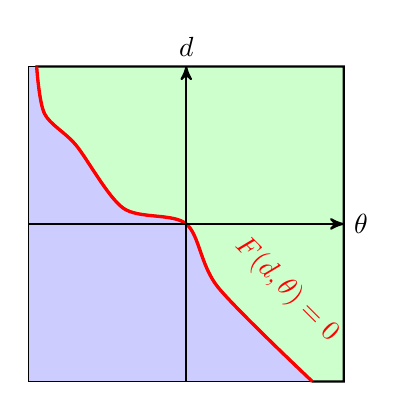
\begin{tikzpicture}[align = center,>=stealth',scale=2]
\tikzstyle{myedge}=[shorten >=1pt,auto,semithick]
\tikzstyle{axes}=[->,opacity = 1.0]
\coordinate (A) at (0,0);
\draw[fill=blue!20] (A) +(-1,-1) rectangle +(1,1);
\def\cxyline{(0.8,-1) (0.2,-0.4) (-0,0) (-0.4,0.1) (-0.7,0.5)  (-0.9,0.7) (-0.95,1)}
\draw [thick, name = cxyline,fill = green!20] plot [smooth] coordinates {\cxyline } -- (1,1) -- (1,-1) -- cycle;
\draw[very thick, red] plot [smooth] coordinates {\cxyline } (A)++(-45:0.25) node[above right,rotate=-45]{$F(d,\theta)=0$};
\draw[->,thick] (A) +(-1,0) -- +(1,0) node[right] {$\theta$};
\draw[->,thick] (A) +(0,-1) -- +(0,1) node[above] {$d$};
\end{tikzpicture}
    \caption{A depiction of the line $F(d,\theta) = 0$}
    \label{fig:my_label}
\end{figure}


\begin{align}
    \label{eq:ls-dbound} \invf{h}(\tlb) &\le \dlb < 0 < \dub \le \invf{h}(\dub) \\
    \label{eq:ls-tbound} -\pi &< \tlb < 0 < \tub < \pi \\
    \label{eq:ls-qone} \Qone &\triangleq \left\{ (\theta,d) : \theta\in(0,\tub), d\in[0,\dub) \right\} \\
    \label{eq:ls-qtwo} \Qtwo &\triangleq \left\{ (\theta,d) : \theta\in(\tlb, 0], d\in(0,\dub) \right\} \\
    \label{eq:ls-qthr} \Qthr &\triangleq \left\{ (\theta,d) : \theta\in(\tlb, 0), d\in(\dlb,0] \right\} \\
    \label{eq:ls-qfor} \Qfor &\triangleq \left\{ (\theta,d) : \theta\in[0,\tub), d\in(\dlb,0) \right\} \\
    \label{eq:ls-qone-line} \Qoneic &\triangleq \left\{ (\theta,d) : (\theta,d)\in\Qone, d\le -\frac{\dub}{\tub}\theta + \dub \right\} \\
    \label{eq:ls-qthr-line} \Qthric &\triangleq \left\{ (\theta,d) : (\theta,d)\in\Qthr, d\le -\frac{\dlb}{\tlb}\theta + \dlb \right\} \\
    \label{eq:ls-Xo} \Xo &\triangleq \Qoneic \cup \Qtwo \cup \Qthric \cup \Qfor \\
    \label{eq:ls-X} X &\triangleq \Xo \cup \Qone \cup \Qthr \\
    \label{eq:traj-with-ic} \vx(t;\vxz) &= \vxz + \int_0^t \dot\vx(\tau) d\tau
\end{align}


\subsection{LS Stability}
\begin{fact}
\label{fact:ls-stability}
    Let $\vxz\in\Xo$.
    Then, $\exists 0 < \alpha, \beta, \gamma < \infty$ s.t. the control laws~\eqref{eq:omega-ctrl-law} and~\eqref{eq:v-ctrl-law} ensure that, $\forall t>0$, $\vx(t)\in X$.\todo{BC: Change conditions to $\alpha \ge 0$}
\end{fact}


\begin{proof}
\emph{Quadrant 1}:
    Let $\vxz \in \Qoneic$.
    Define $L_1 \triangleq \Qoneic\cap\left\{ d = -\frac{\dub}{\tub}\theta + \dub  \right\}$ and $L_3 \triangleq \Qthric\cap\left\{ d = -\frac{\dlb}{\tlb}\theta - \dlb  \right\}$ similar to the proof of Fact~\ref{fact:d-axis-crossing}.
    Select
    \[ \uF = \min_{\vx\in(L_1\cup L_3)} |F(\vx)|, \]
    and let $\alpha,\beta,\gamma > 0$ such that
    \[ \frac{\beta'}{\gamma} < \uF \cdot \min\left\{ \frac{\dub}{\tub}, \frac{\dlb}{\tlb} \right\}. \]
    Fact~\ref{fact:d-axis-crossing} shows that with the choice of hyper-parameters listed previously, $\forall \vxz\in\Qoneic$, $\exists t < \infty$ s.t. $\vx(t;\vxz)\in\Qtwo$, where $\forall t'<t$, $\vx(t';\vxz)\in\Qone$.

    \emph{Quadrant 2}:
    Starting on the $d$ axis, note that $\forall \vxz\in\{(0,d) : d > 0 \}$, $\dot \theta < 0$ and $\dot d = 0$.
    Thus, we must enter $\Qtwo\setminus\left\{ (0,d) : d > 0 \right\}$.
    %Once in $\Qtk$ the proof is rather simple.
    Once in $\Qtwo\setminus\left\{ (0,d) : d > 0 \right\}$ the proof is rather simple.
    $\forall\vxz\in\Qtwo\setminus\left\{ (0,d) : d > 0 \right\}$, $\dot d < 0$, and on either side of the line $F(\theta,d) = 0$, $\dot\theta$ pushes us back towards this line.
    This ensures our trajectory $\vx(t;\vxz)$ remains bounded in $\Qtwo$ or exits across the $\theta$ axis into quadrant 3 along the line 
    $L_2 \triangleq \left\{(\theta,0) : \theta\in(\tlb,0) \right\}$.
    If we do not ever cross the axis, then we either remain in $\Qtwo$ for all time, or we are driven to the equilibrium.
    If we cross the $\theta$ axis within $L_2$, given our selection of $\alpha,\beta,\gamma$, the same argument given above for quadrants 1 and 2 holds for quadrants 3 and 4.
    While there is no guarantee of the trajectory heading towards $\vxe$, this does imply that $\forall t, \vx(t;\vxz)\in X$.
    In essence, if we cross the $\theta$ axis along $L_2$, we will be guaranteed to at least re-enter $X_0$ if it does not go to the equilibrium.
    This concludes the proof.
\end{proof}

\begin{remark}
Fact~\ref{fact:ls-stability} can be rewritten to show that $\exists 0<\alpha,\beta,\gamma<\infty$ s.t. control laws~\eqref{eq:omega-ctrl-law} and~\eqref{eq:v-ctrl-law} make the mobile robot a Lyapunov stable system using a slightly more restrictive initial condition set.
Define $X = \left\{ (\theta,d) | \theta\in(\tlb,\tub), d\in(\dlb,\dub) \right\}\setminus\{ (0,0) \}$.
Then, Fact~\ref{fact:ls-stability} implies that $\forall \epsilon>0$, $\exists \delta>0$ s.t. 
\[ || \vxz - \vxe ||_1 < \delta \implies || \vx(t;\vxz) - \vxe ||_\infty < \epsilon \]
$\forall t \ge 0$.\todo{BC: This isn't quite right, as I need to make $X$ a perfect square. This should be a good starting point for what may be interesting to show though.}
\end{remark}

\begin{fact}
    \label{fact:d-axis-crossing}
    Let $\vxz\in\Qoneic$.
    Then, $\exists 0<\alpha,\beta,\gamma<\infty$ such that the following two conditions hold:
    \begin{enumerate}
        \item \label{fact:d-axis-crossing-cond1} $\exists t<\infty$ s.t. $\vx(t;\vxz) = [0,d(t)]^\intercal$, where $d(t)<\dub$, and
        \item \label{fact:d-axis-crossing-cond2} $\forall t'<t$, $\vx(t';\vxz) \in \Qone$.
    \end{enumerate}
\end{fact}


\begin{proof}
We begin by showing the hyper-parameter selection needed to guarantee condition~\ref{fact:d-axis-crossing-cond1} holds.
Fact~\ref{fact:finite-time} shows that $\forall \vxz\in\Qoneic$, $\exists t<\infty$ such that $\theta(t) = 0$.
Let $t$ be this finite choice, and thus we know $\vx(t;\vxz) = [0, d(t)]^\intercal$.
All that remains to show is that our hyper-parameter selection will guarantee $d(t) < \dub$.

To begin, we denote the line $L_1 \triangleq \Qoneic\cap\left\{ d = -\frac{\dub}{\tub}\theta + \dub  \right\}$.
Note that all initial conditions along $L_1$ takes the form
\[ (\theta_0,d_0) = \left(\theta_0, -\frac{\dub}{\tub}\theta_0 + \dub\right). \]
In essence, what we need to show is that for the given $t$ corresponding to $\theta(t) = 0$,
\[ d(t) = d_0 + \int_0^t \dot d(\tau) d\tau < \dub. \]
First, let $-\uF = \max_{\vx\in L_1} F(\vx)$, which corresponds to the smallest negative value $F$ can take along or above this line.
%Next, we note that $\forall \alpha>0$, $F < \uF < 0$, the following bound holds
Next, fix $\alpha > 0$.
The selection of both $\alpha$ and $-\uF$ allow $\dot d$ to be bounded as
\[ \dot d(t) \le \beta e^{-\alpha(-\uF)^2}\sin(\theta(t)). \]
Since $\alpha$ and $\uF$ are fixed values, we can denote this as a constant $\beta' = \beta e^{-\alpha\uF^2}$.

For each trajectory $\vx(t;\vxz)$, there are two possible outcomes:
\begin{enumerate}
    \item $\vx(t;\vxz)$ remains below the line $L_1$, or
    \item $\vx(t;\vxz)$ lies on or above the line at some point in time.
\end{enumerate}
If the first condition is satisfied, we clearly must cross below the point $d(t) = \dub$, which concludes the proof.
Thus, we will assume the opposite holds.

Since $\vx(t;\vxz)$ is on or above the line, $F(\vx) \le \uF$.
The function $F$ can also be reparameterized as a function of the initial conditions and time as $F(\vx(t)) = F(t;\vxz)$.
Lastly, note that $\forall \vx\in\Qone$, $F(\vx(t)) < 0$.
These facts allow the bound to be reparameterized in the following way:
\begin{align*}
    d(t) &= d_0 + \int_0^t \beta e^{-\alpha F^2}\sin\theta(\tau)d\tau \\
    &\le d_0 + \int_0^t \beta'\sin\theta(\tau)d\tau \\
    &= d_0 + \int_0^t \beta'\sin\theta(\tau)\frac{\gamma F(\tau;\vxz)}{\gamma F(\tau;\vxz)}d\tau \\
    &\le d_0 + \int_0^t \frac{1}{\gamma(-\uF)} \beta'\sin\theta(\tau) \gamma F(\tau;\vxz) d\tau \\
    &= d_0 + \frac{\beta'}{\gamma(-\uF)} \int_0^t \sin\theta(\tau)\gamma F(\tau;\vxz)d\tau
\end{align*}
Note that $\forall t$, $\sin\theta(t) > 0$ and $F(t;\vxz) < 0$, implying that the integral term must be less than zero.
Thus, to avoid later sign confusion, the bound is simplified as
\[ d(t) \le d_0 + \frac{\beta'}{\gamma\uF} \int_0^t \sin\theta(\tau)\gamma F(\tau;\vxz)d\tau, \]
where $\uF > 0$.

We will now make the following substitutions:
\begin{itemize}
    \item $u = \theta$
    \item $du = \dot \theta d\tau = \gamma F(\tau;\vxz)d\tau$
    \item $\theta(0) = \theta_0$
    \item $\theta(T) = 0$.
\end{itemize}
The bound is now simplified to
\begin{align*}
    d(t) &\le d_0 + \frac{\beta'}{\gamma\uF} \int_{\theta_0}^0 \sin u\,du \\
    &= d_0 + \frac{\beta'}{\gamma\uF} (1 - \cos\theta_0).
\end{align*}

Now the final part is to show $\exists \beta,\gamma$ s.t. $\forall d_0\in\Qoneic$, $d(t;d_0) < \dub$.
\begin{align*}
    d(t) &\le d_0 + \frac{\beta'}{\gamma\uF} (1-\cos\theta_0)\\
    &= -\frac{\dub}{\tub}\theta_0 + \dub + \frac{\beta'}{\gamma\uF} (1-\cos\theta_0).
\end{align*}
Note that $\forall \theta_0\in\Qone$, $1-\cos\theta_0 \le \theta_0$.
This turns the final bound into
\begin{align}
    \label{eq:d-final-bound}
    d(t) &\le -\frac{\dub}{\tub}\theta_0 + \dub + \frac{\beta'}{\gamma\uF}\theta_0 \\ \nonumber
    &= \left( \frac{\beta'}{\gamma\uF} - \frac{\dub}{\tub} \right)\theta_0 + \dub.
\end{align}
Equation~\eqref{eq:d-final-bound} must remain less than $\dub\ \forall\theta_0\in\Qone$, implying
\[ \frac{\beta'}{\gamma} < \frac{\dub\uF}{\tub}. \]
Since $\tub, \dub$, and $\uF$ are all finite and positive, this concludes the proof of the first condition.

The second condition can be proven in the following way.
%To begin, note that $(\XL\cap\Qop)\subset\Qok$.
To begin, note that $\Qoneic\subset\Qone$.
We select $\frac{\beta'}{\gamma} < \frac{\dub\uF}{\tub}$, which implies that we must cross the $\theta$ axis below the point $[0,\dub]^\intercal$.
Since $\dot\theta < 0$, we cannot leave $\Qone$ along the $\theta$ direction unless we cross the $\theta$ axis.
Likewise, since $d(t) < \dub$ and $\dot d > 0$, this implies that $\forall t' < t, d(t') < d(t) < \dub$.
Thus, given our choice of $\alpha$, $\beta$, and $\gamma$, $\vx(t',\vxz)\in\Qone$, $0\le t' < t$.
\end{proof}

% \begin{remark}
% The bound
% \[ \frac{\beta'}{\gamma} < \frac{\oF}{k} \]
% has physically insightful meaning between both $\oF$ and $k$.
% For a fixed $\gamma$, as $\oF\rightarrow 0$, $\beta\rightarrow 0$.
% This implies that as our smallest $F$ value in a bounded region decreases, we need to decrease the forward velocity gain $\beta$ to compensate for the slower turning speed $\dot\theta = \gamma F$.
% Similarly, for a fixed $\gamma$, as $k\rightarrow\infty$, $\beta\rightarrow\infty$.
% This implies that as our bound on the desired $d(t)$ value grows, we can increase our forward velocity gain $\beta$ while still maintaining our ultimate bound on $d(t)$ when crossing the $\theta$ axis.\todo{BC: Add remarks about selection of $\alpha$ in here too.}
% \end{remark}


\begin{fact}
\label{fact:finite-time}
Let $0 < \alpha, \beta, \gamma < \infty$.
Then, $\forall \vxz \in \Qoneic$, $\exists t<\infty$ s.t. $\vx (t;\vxz) = [ 0, d(t) ]^\intercal$.
\end{fact}

\begin{proof}
Let $0 < \alpha, \beta, \gamma < \infty$.
For $[\theta_0, d_0]^\intercal = \vxz\in\Qoneic \setminus \{ (\theta, 0) : \theta\in(0,\tub) \}$, conditions~\eqref{eq:delfd} and~\eqref{eq:delft} in conjunction with control laws~\eqref{eq:v-control-law} and~\eqref{eq:w-control-law} imply that, $\forall t$ s.t. $\vx(t;\vxz)\in\Qoneic$:
\[ 0 < F(0,d_0) < F(\theta(t), d(t)). \]
Let $\underline{F} = F(0,d_0)$.
Thus, for any of these initial conditions, it satisfies
\begin{align*}
    \theta(t) &= \theta_0 + \int_0^t \dot \theta d\tau \\
    &\le \theta_0 + \int_0^t \gamma\underline{F} d\tau \\
    &= \theta_0 + \gamma\underline{F} t.
\end{align*}
Let $t = -\frac{\theta_0}{\gamma\underline{F}}<\infty$, and note that $\theta(t) \le 0$ and that $t$ is finite.

For the elements along the line $\vxz\in \{ (\theta,0) : \theta\in(0,\tub) \}$, $\dot d > 0$.
Thus, all points along this line must enter into the set $\Qoneic \setminus \{ (\theta,0) \}$, concluding the proof.


% Note that $\forall \vxz$, $\dot d > 0$.
% Thus, we must enter $\Qonenot$.
% In $\Qop$, note that $\dot d > 0$ and $\dot\theta < 0$.
% Let $[\theta_1, d_1]^\intercal = \vx_1\in\Qop$, and we let $-\oF = F(0,d_1)$, where $\oF > 0$.
% %Conditions~\eqref{eq:delfx} and~\eqref{eq:delft} imply that $\forall \vx_1\in\Qok, \dot \theta \le -\gamma\oF$.
% Conditions~\eqref{eq:delfx} and~\eqref{eq:delft} imply that for our given choice of $\vx_1$ and $\oF$, if $\vx(t;\vx_1)\in\Qone$, $\dot \theta \le -\gamma\oF$.
% This implies the following:
% \begin{align*}
%     \theta(t) &= \theta_1 + \int_0^t \dot \theta d\tau \\
%     &\le \theta_1 + \int_0^t -\gamma\oF d\tau \\
%     &= \theta_1 - \gamma\oF t.
% \end{align*}
% Let $t = \frac{\theta_1}{\gamma\oF}<\infty$, and note that $\theta(t) \le 0$.
% Since $t$ is finite, this concludes the proof.
\end{proof}






% \section{OLD LS Analysis}
% Preliminaries:
% \begin{align}
%     \label{eq:ddot} \dot d &= \beta e^{-\alpha F^2}\sin\theta \\
%     \label{eq:tdot} \dot \theta &= \gamma F \\
%     \label{eq:tbound} \tbound &\in (0,\pi) \\
%     \label{eq:dbound} \dbound &\in(0,h^{-1}(\pi)) \\
%     \label{eq:xlplus} \XLp &\triangleq \{ (\theta, d): d \le -\frac{\dbound}{\tbound}\theta + \dbound \} \\
%     \label{eq:xlminus} \Xlm &\triangleq \{ (\theta, d): d \le -\frac{\dbound}{\tbound}\theta - \dbound \} \\
%     \label{eq:qone} \Qone &\triangleq \{ (\theta, d) : \theta\in (0,\tbound), d\in(0,\dbound) \} \\
%     \label{eq:qtwo} \Qtwo &\triangleq \{ (\theta, d) : \theta\in (-\tbound,0), d\in(0,\dbound) \} \\
%     \label{eq:qthr} \Qthr &\triangleq \{ (\theta, d) : \theta\in (-\tbound,0), d\in(-\dbound,0) \} \\
%     \label{eq:qfor} \Qfor &\triangleq \{ (\theta, d) : \theta\in (0,\tbound), d\in(-\dbound,0) \} \\
%     \label{eq:levelsetcont} \Qonenot &\triangleq \Qone\cap\XLp \\
%     \label{eq:levelsetcontneg} \Qthrnot &\triangleq \Qthr\cap\XLm  \\
%     \label{eq:Forigin} F(\vec 0) &= 0 \\
%     \label{eq:delfd} \frac{\partial F}{\partial d} &< 0\qquad\forall -\dbound \le d \le \dbound \\
%     \label{eq:delft} \frac{\partial F}{\partial \theta} &< 0\qquad\forall -\tbound\le\theta\le\tbound\\
%     \label{eq:traj} \vec x(t;\vec x_0) &= \vec x_0 + \int_0^t \dot{\vec x}(\tau)d\tau \\
% \end{align}
% \clonelabel{eq:ls-prelims-start}{eq:ddot}
% \clonelabel{eq:ls-prelims-end}{eq:traj}
% \clonelabel{eq:F-conds-begin}{eq:Forigin}
% \clonelabel{eq:F-conds-end}{eq:delft}


% \begin{fact}
%     Let $\tbound\in(0,\pi)$ and $\dbound\in(0,\invf{h}(\tbound))$.
%     Let $\vxz\in\left( \Qonenot\cup\Qtwo\cup\Qthrnot\cup\Qfor \right)$.
%     Then, $\exists 0 < \alpha, \beta, \gamma < \infty$ s.t. the control laws~\eqref{eq:ddot} and~\eqref{eq:tdot} ensure that, $\forall t>0$, $\vx(t)\in\left( 
%  \Qone\cup\Qtwo\cup\Qthr\cup\Qfor \right)$.
% \end{fact}


% \begin{proof}
% \emph{Quadrant 1}:
%     Let $\vxz \in X_0$, let $-\oF = \max_{(\theta,x)\in\XL\cap\Qop} F(\theta,x)$ and let $\alpha,\beta,\gamma > 0$, $\frac{\beta}{\gamma} > \frac{\oF}{\theta_0^\star k}$.
%     Since $\dot d > 0$, we must enter $\XLo$.
%     Let $\vx_1\in\XLo$.
%     With our selection $\alpha, \beta$, and $\gamma$, facts~\ref{fact:d-axis-crossing} and~\ref{fact:finite-time} show that $\vx_1$ must cross the $d$ axis below the point $[0,\frac{\pi}{k}]^\intercal$ in finite time while staying within the bounded set $\Qok$.

%     \emph{Quadrant 2}:
%     Starting on the $d$ axis, note that $\forall \vxz\in\{(0,d) : d > 0 \}$, $\dot \theta < 0$.
%     Thus, we must enter $\Qtk$.
%     Once in $\Qtk$ the proof is rather simple.
%     $\forall\vxz\in\Qtk$, $\dot d < 0$, and on either side of $g(\theta,x) = 0$, $\dot\theta$ pushes us towards this line.
%     This ensures our trajectory $\vx(t;\vxz)$ remains bounded in $\Qtk$ or exits across the $\theta$ axis into quadrant 3 along the set $-X_0 \triangleq \{(\theta,0) : -\pi < \theta < 0 \}$.
%     If we cross the $\theta$ axis within $-X_0$, since $F$ is symmetric, everything above applies similarly, although the signs are reversed.
%     In essence, if we cross the $\theta$ axis along $-X_0$, we will be guaranteed to at least re-enter $X_0$ if it does not go to the equilibrium.
%     If we do not ever cross the axis, then we either remain in $\Qtk$ for all time, or we are driven to the equilibrium.

%     We summarize the proof in the following way:
%     If we begin in the set $\XLo \cup \Qtk \cup \{ (0,d) : 0 < d < \frac{\pi}{k} \}$ (or it's counterpart flipped across the $\theta$ axis), we will remain bounded in the set $\{ (\theta, d) : \theta\in(-\pi,\pi), d\in(-\frac{\pi}{k},\frac{\pi}{k}) \}$.
% \end{proof}


% \begin{fact}
%     \label{fact:d-axis-crossing}
%     Let $\vxz\in\XL^+\cap\Qone$.
%     Then, $\exists 0<\alpha,\beta,\gamma<\infty$ such that the following two conditions hold:
%     \begin{enumerate}
%         \item \label{fact:d-axis-crossing-cond1} $\exists t<\infty$ s.t. $\vx(t;\vxz) = [0,d(t)]^\intercal$, where $d(t)<\frac{\pi}{k}$, and
%         \item \label{fact:d-axis-crossing-cond2} $\forall t'<t$, $\vx(t';\vxz) \in \Qok$.
%     \end{enumerate}
% \end{fact}

% \begin{proof}
% We begin by showing the hyper-parameter selection needed to guarantee condition~\ref{fact:d-axis-crossing-cond1} holds.
% Fact~\ref{fact:finite-time} shows that $\forall \vxz\in X_0\cup\Qone$, $\exists t<\infty$ such that $\theta(t) = 0$.
% Let $t$ be this finite choice, and thus we know $\vx(t;\vxz) = [0, d(t)]^\intercal$.
% All that remains to show is that our hyper-parameter selection will guarantee $d(t) < \frac{\pi}{k}$.

% To begin, we note that all initial conditions along the line $\XL\cap\Qop$ takes the form
% \[ (\theta_0,d_0) = \left(\theta_0, \frac{\pi - \theta_0}{k}\right). \]
% In essence, what we need to show is that for the given $T$ corresponding to $\theta(T) = 0$,
% \[ d(T) = d_0 + \int_0^T \dot d(\tau) d\tau < \frac{\pi}{k}. \]
% First, let $-\oF = \max_{(\theta,d)\in\XL\cap\Qone} F(\theta,x)$, which corresponds to the smallest negative value $F$ can take along or above this line.
% Next, we note that $\forall \alpha>0$, $F < -\oF$, the following bound holds
% \[ \dot d(t) \le \beta e^{-\alpha\oF^2}\sin(\theta(t)). \]
% Since $\alpha$ and $\oF$ are fixed values, we can denote this as a constant $\beta' = \beta e^{-\alpha\oF^2}$.

% For each $\vx(t;\vxz)$, there are two possible conditions:
% \begin{enumerate}
%     \item $\vx(t;\vxz)$ remains below the line $\XL\cap\Qone$, and
%     \item $\vx(t;\vxz)$ goes above the line at some point in time.
% \end{enumerate}
% If the first condition is satisfied, we clearly must cross below the point $d(t) = \frac{\pi}{k}$, which concludes the proof.
% Thus, we will assume the opposite holds.

% Since $\vx(t;\vxz)$ is above the line, we know everywhere above this line, $-F(\vx) < -\oF$.
% We can use this fact to reparameterize our bound in the following way:
% \begin{align}
%     d(T) &= d_0 + \int_0^T \beta e^{-\alpha F^2}\sin\theta(\tau)d\tau \\
%     &\le d_0 + \int_0^T \beta'\sin\theta(\tau)d\tau \\
%     &= d_0 + \int_0^T \beta'\sin\theta(\tau)\frac{\gamma F(\tau)}{\gamma F(\tau)}d\tau \\
%     &\le d_0 + \int_0^T \frac{1}{\gamma\oF} \beta'\sin\theta(\tau) \gamma F(\tau) d\tau \\
%     &= d_0 + \frac{\beta'}{\gamma\oF} \int_0^T \sin\theta(\tau)\gamma F(\tau)d\tau
% \end{align}
% We will now make the following substitutions:
% \begin{itemize}
%     \item $u = \theta$
%     \item $du = \dot \theta d\tau = \gamma F(\tau)d\tau$
%     \item $\theta(0) = \theta_0$
%     \item $\theta(T) = 0$.
% \end{itemize}
% The bound is now simplified to
% \begin{align}
%     d(t) &\le d_0 + \frac{\beta'}{\gamma\oF} \int_{\theta_0}^0 \sin u\,du \\
%     &= d_0 + \frac{\beta'}{\gamma\oF} (1 - \cos\theta_0).
% \end{align}

% Now the final part is to show $\exists \beta,\gamma$ s.t. $\forall d_0\in\XL\cap\Qop$, $d(t;d_0) < \frac{\pi}{k}$.
% \begin{align}
%     d(t) &\le d_0 + \frac{\beta'}{\gamma\oF} (1-\cos\theta_0)\\
%     &= \frac{\pi - \theta_0}{k} + \frac{\beta'}{\gamma\oF} (1-\cos\theta_0).
% \end{align}
% Note that $\forall \theta_0\in X_0$, $1-\cos\theta_0 \le \theta_0$.
% This turns the final bound into
% \begin{align}
%     d(t) &\le \frac{\pi - \theta_0}{k} + \frac{\beta'}{\gamma\oF} \theta_0 < \frac{\pi}{k}\\
%     &\implies \frac{\beta'}{\gamma} < \frac{\oF}{k},
% \end{align}
% where $\oF$ and $k$ are finite.
% Thus,
% \[ \frac{\beta'}{\gamma} < \frac{\oF}{k} \implies \forall \vxz\in\XL\cap\Qop, d(t;d_0) < \frac{\pi}{k}. \]

% We have now proven the first condition in the fact.
% The second condition can be proven in the following way.
% To begin, note that $(\XL\cap\Qop)\subset\Qok$.
% We select $\frac{\beta'}{\gamma} < \frac{\oF}{k}$, which implies that we must cross the $\theta$ axis below the point $[0,\frac{\pi}{k}]^\intercal$.
% Since $\dot\theta < 0$, we cannot leave $\Qok$ along the $\theta$ direction unless we cross the $\theta$ axis.
% Likewise, since $d(t) < \frac{\pi}{k}$ and $\dot d > 0$, this implies that $\forall t' < t, d(t') < d(t) < \frac{\pi}{k}$.
% Thus, given our choice of $\alpha$, $\beta$, and $\gamma$, $\vx(t',\vxz)\in\Qok$, $0\le t' < t$.
% \end{proof}

% \begin{remark}
% The bound
% \[ \frac{\beta'}{\gamma} < \frac{\oF}{k} \]
% has physically insightful meaning between both $\oF$ and $k$.
% For a fixed $\gamma$, as $\oF\rightarrow 0$, $\beta\rightarrow 0$.
% This implies that as our smallest $F$ value in a bounded region decreases, we need to decrease the forward velocity gain $\beta$ to compensate for the slower turning speed $\dot\theta = \gamma F$.
% Similarly, for a fixed $\gamma$, as $k\rightarrow\infty$, $\beta\rightarrow\infty$.
% This implies that as our bound on the desired $d(t)$ value grows, we can increase our forward velocity gain $\beta$ while still maintaining our ultimate bound on $d(t)$ when crossing the $\theta$ axis.\todo{BC: Add remarks about selection of $\alpha$ in here too.}
% \end{remark}


% \begin{fact}
% \label{fact:finite-time}
% Let $0 < \alpha, \beta, \gamma < \infty$.
% Then, $\forall \vxz \in X_0\cup\Qonenot$, $\exists t<\infty$ s.t. $\vx (t;\vxz) = [ 0, d(t) ]^\intercal$.
% \end{fact}

% \begin{proof}
% Let $0 < \alpha, \beta, \gamma < \infty$, and $\vxz \in X_0$.
% Note that $\forall \vxz$, $\dot d > 0$.
% Thus, we must enter $\Qonenot$.
% In $\Qop$, note that $\dot d > 0$ and $\dot\theta < 0$.
% Let $[\theta_1, d_1]^\intercal = \vx_1\in\Qop$, and we let $-\oF = F(0,d_1)$, where $\oF > 0$.
% %Conditions~\eqref{eq:delfx} and~\eqref{eq:delft} imply that $\forall \vx_1\in\Qok, \dot \theta \le -\gamma\oF$.
% Conditions~\eqref{eq:delfx} and~\eqref{eq:delft} imply that for our given choice of $\vx_1$ and $\oF$, if $\vx(t;\vx_1)\in\Qone$, $\dot \theta \le -\gamma\oF$.
% This implies the following:
% \begin{align*}
%     \theta(t) &= \theta_1 + \int_0^t \dot \theta d\tau \\
%     &\le \theta_1 + \int_0^t -\gamma\oF d\tau \\
%     &= \theta_1 - \gamma\oF t.
% \end{align*}
% Let $t = \frac{\theta_1}{\gamma\oF}<\infty$, and note that $\theta(t) \le 0$.
% Since $t$ is finite, this concludes the proof.
% \end{proof}



\subsection{LAS Analysis}
Preliminaries (include preliminaries~\eqref{eq:ls-prelims-start}---~\eqref{eq:ls-prelims-end}):
\begin{align}
    \label{eq:F0} F_0 &\triangleq \{ (\theta,d) : F(\theta,d) = 0 \} \\
    %\label{eq:Fh} F_h(\theta) &\triangleq F(\theta, h(\theta))\text{ s.t. } (\theta,h(\theta))\in F_0\\
    \label{eq:FL} F_L(\theta) &\triangleq F\left(\theta, -L\theta \right)
\end{align}



\begin{fact}
    There exists $\alpha, \beta, \gamma > 0$ such that, $\forall \vxz\in X_0$, $\lim_{t\rightarrow\infty}\vx(t;\vxz) = 0$.
\end{fact}

\begin{proof}
    Let $L$ satisfy Fact~\ref{fact:L-bound}.
    Let $\alpha > 0$ and $\frac{\beta}{\gamma}$ satisfy facts~\ref{fact:d-axis-crossing} and~\ref{fact:L-vf-bound} according to the $L$ chosen previously.

    We begin this proof by incorporating previous results from the proof of Fact~\ref{fact:ls-stability}.
    This fact showed that, $\forall \vxz\in\Qone$, we will enter $\Qtwo$ below the point $\dub$ and pass through the line $F_0$.
\end{proof}



\begin{fact}
\label{fact:L-vf-bound}
%Let $-\theta\in(-\tbound, 0)$, and define $L$ based on Fact~\ref{fact:L-bound}.
Define $L$ based on Fact~\ref{fact:L-bound}.
Denote the line $L$ makes in quadrant two as $L_2\triangleq\Qtwo\cap\{ (\theta,d) : d = -L\theta \}$
Then, $\exists \alpha,\beta,\gamma > 0$ such that, $\forall (\theta,d)\in L_2$, the following inequality holds:
\[ \tan{\left(-L\right)} \le \tan{\left( \frac{\dot d}{\dot\theta} \right)}. \]
\end{fact}

\begin{proof}
We begin the proof as
    \begin{align*}
        \tan{\left( -L \right)} &\le \tan{\left( \frac{\dot d}{\dot\theta} \right)} \\
        \implies -L &\le \frac{\dot d}{\dot\theta} \\
        \implies -\dot\theta L &\le \dot d \\
        \implies -\gamma F_L(\theta) L &\le \beta e^{-\alpha F_L^2(\theta)}\sin(-\theta)\\
        \implies \gamma F_L(\theta) L &\ge \beta\sin(\theta) \ge \beta e^{-\alpha F_L^2(\theta)}\sin(\theta)\\
        \implies \frac{\gamma}{\beta} &\ge \frac{1}{L} \frac{\sin(\theta)}{F_L(\theta)} \\
        \implies \frac{\beta}{\gamma} &\le \frac{L F_L(\theta)}{\sin(\theta)}.
    \end{align*}
    The last inequality holds since our choice of $L$ guarantees that $F_L(\theta)$ remains positive along that line.
    The last thing to show is that the fraction $\frac{F_L(\theta)}{\sin\theta}$ remains bounded as $\theta\rightarrow 0$. \todo{Find the minimum of $\frac{F_L(\theta)}{\sin\theta}$ over $\theta$ in an interval and show that it is strictly positive}
    For this we will use L'Hopital's rule.
    \begin{align*}
    \lim_{\theta\rightarrow 0} \frac{F_L(\theta)}{\sin\theta} &= \frac{0}{0}\\
    \implies \lim_{\theta\rightarrow 0} \frac{F_L(\theta)}{\sin\theta} &= \lim_{\theta\rightarrow 0} \frac{F_L'(\theta)}{\cos\theta}\\
    \implies \lim_{\theta\rightarrow 0} \frac{F_L(\theta)}{\sin\theta} &= F_L'(0).
    \end{align*}
    Note that, by the choice of $L$ and conditions ... and ..., $0 < F'_L(\theta) < \infty$. \todo{have you determined these conditions?} 

    Finally, select 
    \[ \frac{\gamma}{\beta} = L\cdot\inf_{\theta\in L2}\left( \frac{F_L(\theta)}{\sin\theta} \right). \]
    Since the hyper-parameter choice is positive and finite, it concludes the proof.
\end{proof}


\begin{fact}
\label{fact:L-bound}
    %Let $\theta\in(\tlb, 0)$.
    %Then, $\exists L>0$ such that $\forall d\in F_0\cap\Qtwo$, $d \ge -L\theta$.
    $\exists L>0$ such that the following two conditions are met:
    \begin{align}
        &\forall d\in F_0\cap\Qtwo, d \ge -L\theta, \text{ and},\\
        &\forall d\in F_0\cap\Qfor, d \le -L\theta.
    \end{align}
\end{fact}

\begin{proof}
    We begin the proof by showing that the first condition holds.
    If so, the second condition can be shown to hold by an argument of symmetry.
    Note that this symmetry does not imply that the maximum $L$ is the same for both conditions, but rather, if $L'$ satisfies the first and $L''$ satisfies the second, then $L=\min\{ L', L''\}$ satisfies both.
    Thus we aim to prove the first condition true, and the second follows by symmetry.
    
    Conditions $\frac{\partial{F}}{\partial{\theta}} < 0$ and $\frac{\partial{F}}{\partial{\theta}} < 0$ in conjunction with the Implicit Function Theorem imply that the graph of $F_0$ can be represented by a function $h(\theta) = d$, where $h$ has the following properties:
    \begin{itemize}
        \item $h$ exists along the entire domain of $F_0$,
        \item $h$ is strictly monotonically decreasing,
        \item $h(0) = 0$, and
        \item $\forall\theta,\, h'(\theta) < 0$.
    \end{itemize}
    With these properties, a trivial bound of $F_0$ is $L=0$, as the monotonicity of $h$ implies that $h(\theta) \ge 0\ \forall\theta\in(\tlb,0)$.
    However, we would like to show that there is a non-zero lower bound on this function.
    Let $L > 0$.
    Then
    \begin{align*}
        h(\theta) &\ge -L\theta \\
        \implies \frac{h(\theta)}{\theta} &\le -L \ (\text{due to the fact that } \theta < 0) \\
        \implies \frac{h(\theta)}{-\theta} &\ge L.
    \end{align*}
    Note that since $\theta<0$, $\frac{h(\theta)}{-\theta} > 0$.

    To ensure that $L$ bounds all values, two conditions are required.
    These conditions are
    \begin{align}
        \lim_{\theta\rightarrow0}\frac{h(\theta)}{-\theta} &\ne 0,\text{ and}\\
        \min_{\theta\in\Qtwo} \frac{h(\theta)}{-\theta} &> 0
    \end{align}
    If both of these conditions are true, then letting $L$ be the minimum of these two conditions will ensure the bound is valid, implying $L > 0$ exists.
    
    To show the first condition holds, we begin by evaluating the limit.
    This limit evaluates to
    \begin{equation*}
        \lim_{\theta\rightarrow0}\frac{h(\theta)}{-\theta} = \frac{0}{0},
    \end{equation*}
    implying that L'Hopital's rule may be used to evaluate this limit.
    This provides
    \begin{equation*}
        \lim_{\theta\rightarrow0}\frac{h(\theta)}{-\theta} = \lim_{\theta\rightarrow0}\frac{h'(\theta)}{1}.
    \end{equation*}
    Since $h'(\theta) < 0$,
    \begin{equation*}
        \lim_{\theta\rightarrow0}\frac{h(\theta)}{-\theta} \ne 0.
    \end{equation*}

    The second condition comes trivially with the first condition in combination with the strictly monotonically decreasing nature of $h$.
\end{proof}

\section{Lyapunov stability}
We would like to show that there exists a choice of parameters $\alpha,\beta$, and $\gamma$ such that the origin is Lyapunov stable.
We first begin by proving the following supporting lemma.
\begin{lemma}
\label{lem:boundedd}
    Let $\delta > 0$.
    Let $\vxz\in\icsetone\triangleq\{ \vx\in X\cap\Qone \colon d = \delta, \theta \le \delta \}$.
    Then, $\exists \alpha,\beta,\gamma$, $\epsilon(\alpha,\beta,\gamma)>0$ and $0<T<\infty$ s.t. $\epsilon$ may be made arbitrarily small and the following conditions are satisfied:
    \begin{align*}
        \theta(T) &= 0,\text{ and }\\
        d(T) &< \delta + \epsilon.
    \end{align*}
\end{lemma}

\begin{proof}
By lemma~\ref{lem:coneinfinitetime}, $\exists T>0$ s.t. $\forall\vxz\in\icsetone$, $\theta(T)=0$.
We also note that equations~\eqref{eq:omega-ctrl-law}, \eqref{eq:v-ctrl-law}, \eqref{eq:tdot}, \eqref{eq:ddot} and StBSF conditions~\eqref{eq:stbsfcondzero}-\eqref{eq:stbsfcondpdd} imply that $\forall t < T$, $0 > F(0,\delta) > F(\vx(t;\vxz))$.
We will denote this as $\stbsfov = F(0,\delta)$.

Analysis of the dynamics shows
    \begin{align}
        \nonumber d(T) = d_0 + \int_0^T\dot d dt &< d_0 + \int_0^T\beta dt\\
         \label{eq:dTbound} &= \delta + \beta T.
    \end{align}
    \begin{align}
        \nonumber \theta(T) &= \theta_0 + \int_0^T\dot\theta dt \le \delta + \int_0^T\dot\theta dt\\
        \nonumber &\le \delta + \int_0^T\gamma\stbsfov dt = \delta + \gamma\stbsfov T \\
        &\implies T \le \frac{-\delta\stbsfov}{\gamma}. \label{eq:Tbound}
    \end{align}

Equations~\eqref{eq:dTbound} and~\eqref{eq:Tbound} can be combined to show
\[ d(T) < \delta + \beta T \le \delta + \beta \frac{-\delta\stbsfov}{\gamma}. \]
Letting $\beta = \epsilon\frac{\gamma}{-\delta\stbsfov} \implies d(T) < \delta + \epsilon$.
Likewise, letting $\epsilon(\alpha,\beta,\gamma) = \frac{\beta}{\gamma}(-\delta\stbsfov)$ completes the proof, as the term $-\delta\stbsfov$ is a fixed, positive term, and the parameters $\beta$ and $\gamma$ may be selected to make $\epsilon$ arbitrarily small.
\end{proof}

%\newcommand{\ballinf}[2]{B_{#1}^\infty\left({#2}\right)}
\newcommand{\ballinf}[2]{B_{#1}^\infty({#2})}
\newcommand{\bdelta}{\ballinf{\delta}{\vec 0}}
\newcommand{\beps}{\ballinf{\epsilon}{\vec 0}}
\newcommand{\inftynorm}[1]{||{#1}||_\infty}
We now show that, given certain parameter selection to the control law, the origin of the system is Lyapunov stable.
We first begin by defining an infinity norm ``ball'' (which will be a square in the state space).
\begin{definition}
An $\alpha$-infinity norm ball, centered at a point $\vx$, is the set
\[ \ballinf{\alpha}{\vx} \triangleq \{ \vx'\in X \colon \inftynorm{\vx-\vx'}<\alpha \}. \]
\end{definition}

We now present the lemma for Lyapunov stability.
\begin{lemma}[Lyapunov Stability]
\label{lem:lyap-stab}
$\forall \epsilon > 0$, $\exists \delta(\epsilon)>0$ s.t. $\forall\vxz\in\bdelta$ and $\forall t>0$, $\vx(t;\vxz)\in\beps$.
\end{lemma}

\begin{proof}
    We will show that in each quadrant $\quadrant_i$, $\forall\vxz\in\bdelta\cap \quadrant_i$, $\vx(t;\vxz)\in\beps\cap \quadrant_i$.
    Since $\cup_i \left(\quadrant_i\cap\beps\right) = \beps$, this will imply $\vx(t;\vxz)\in\beps\ \forall t>0$.
    We also argue along the lines of symmetry, that any trajectory occurring in $\Qone$ will have a similar (but sign flipped) trajectory occurring in $\Qthr$, and the same for $\Qtwo$ and $\Qfor$.
    Thus, we will limit our analysis to quadrants $\Qone$ and $\Qtwo$, and the rest follows by symmetry.\newline
    \underline{$\vxz\in\Qone\cap\bdelta$}:  Lemma~\ref{lem:coneinfinitetime} showed that $\forall \vxz\in\Qone$, $\exists T<\infty$ s.t. $\vx(T;\vxz) = [0,d(T)]^\intercal$ for some $d(T)>0$.
    We just need to show that for our choice of $\alpha, \beta, \gamma, \text{ and } \epsilon$, $d(T)<\epsilon$.
    Note that $\forall\vxz\in\Qone\cap\bdelta$, one of two outcomes can occur:
    \begin{enumerate}
        \item $\theta(T) = 0 \implies d(T) < \delta$, $\implies d(T) < \epsilon$, and
        \item $\exists T'<T$ s.t. $\theta(T') > 0$ and $d(T') = \delta$.
    \end{enumerate}
    For the first case, it is already the case that $\vx(t;\vxz)\in\Qone\cap\beps\ \forall t<T$.
    Thus we limit ourselves to the second case.

    Analysis similar to Lemma~\ref{lem:boundedd} shows that we can bound our state value for $d$ as
    \[ d(T) < d(T') + \int_{T'}^T \beta dt = d(T') + \beta (T-T') = \delta + \beta(T-T'). \]
    The same lemma also showed that we may select an arbitrarily small $\epsilon'(\alpha,\beta,\gamma) > 0$ s.t.
    \[ d(T) < \delta + \epsilon'. \]
    Selecting parameters $\beta$ and $\gamma$ s.t. $\epsilon' < \epsilon - \delta$ implies $d(T) < \epsilon$, further implying that $\forall t<T, \vx(t;\vxz)\in\beps\cap\Qone$.\newline
    \underline{$\vxz\in\Qtwo\cap\bdelta$}: First, note that $\forall\vxz\in\Qtwo\cap\bdelta\setminus\{0\}, \dot d < 0$.
    Likewise, note that $\forall d>h(\theta)$, $\dot\theta < 0$, and $\forall d<h(\theta)$, $\dot\theta > 0$.
    These facts imply that any point entering into $\Qtwo$ must do so along the positive $d$-axis, and any point leaving $\Qtwo$ (other than approaching the origin) must do so along the negative $\theta$-axis.
    These facts also imply that for any point crossing into $\Qtwo$ along the point $[0,d_0]^\intercal$, the furthest $\vx(t;\vxz)$ could cross into $\Qthr$ along the $\theta$-axis would occur at $[\invf{h}(d_0),0]^\intercal$.
    The coordinates $[0,d_0]^\intercal$ and $[\invf{h}(d_0),0]^\intercal$ form a box in $\Qtwo$ containing any valid solution $\vx(t;\vxz)$.
    Thus, selecting $\delta=\max\{ d_0, \invf{h}(d_0) \}$ ensures that $\forall t>0$ s.t. $\forall\vx(t;\vxz)\in\Qtwo$, $\vx(t;\vxz)\in\bdelta\cap\Qtwo\subset\beps\cap\Qtwo$.

    As a final note, the bound $\delta$ for $\Qtwo$ relies on the crossing point into $\Qtwo$ from $\Qone$.
    However, to ensure $\delta$ is uniform for all quadrants, we need to ensure that the crossing point $d_0$ can be made arbitarily small.
    Note that by the analysis for quadrant $\Qone$, we can choose any $\delta$ bound and parameters $\beta$ and $\gamma$ such that we remain bounded by any $\epsilon > 0$.
    Thus, we only need to ensure that for $\delta_1$ chosen in $\Qone$ and the $\delta_2$ chosen in $\Qtwo$, $\delta$ satisfies $\delta = \min\{ \delta_1, \delta_2 \}$.
\end{proof}

\begin{remark}
    Lyapunov stability analysis typically involves the use of balls defined on the $L$-2 norm.
    However, due the equivalency of norms, our definition provided above still satisfies the typical definition of Lyapunov stability.
\end{remark}


\section{Line Following Robots}
One application of the proposed continuous control law is the explanation of stability found in line following robots.
A line following robot is a mobile robot that is equipped with two sensors equally spaced on both sides.
These sensors emit a signal depending on whether some characteristic of a line is detected, such as an infrared sensor detecting a black strip along the ground.
Depending upon which sensor picks up the line, a different signal is emitted, such as a $1$ and $-1$ for either sensor, and a $0$ if neither sensor is picking anything up.

Let $\vec v = [v_r, v_l]^\intercal$ be the commanded right and left wheel velocities, respectively.
The typical control scheme for a line following robot is
\begin{equation*}
    \vec v(F)=
    \begin{cases}
        [1,-1]^\intercal & \text{if } F = -1\\
        [1, 1]^\intercal & \text{if } F = 0\\
        [-1,1]^\intercal & \text{if } F = 1
    \end{cases}
\end{equation*}
which corresponds to the following two cases in our state space
\begin{equation*}
    \dot d(F)=
    \begin{cases}
    0 & \text{if } F = 1,-1\\
    2\sin\theta & \text{if } F = 0
    \end{cases}
\end{equation*}
and
\begin{equation*}
    \dot\theta(F)=
    \begin{cases}
        F & \text{if } F = 1,-1\\
        0 & \text{if } F = 0.
    \end{cases}
\end{equation*}

\section{Experiments}
Experiments for this work consist of both simulations and physical experiments.
Both sets of experiments consist of a WMR attached with an on-board depth sensor, wherein a SeBSF was used to control the robot.

\subsection{Obtaining a SeBSF}
\label{sec:experimentsebsf}
A support vector machine~\cite{Cortes1995} (SVM) maps vector-valued inputs $y$ to binary class labels. When these labels are $\{+1,-1\}$ then the SVM is given by 
\[ f(\vy) = \sign{(w^T y + c)}, \]
where $w$ and $c$ are the weights and bias terms of the SVM. %
We obtain an SeBSF by training an SVM using labeled data, and then using the argument of the $\sign{}$ function as the sensor-based score: 
\begin{align}
    \sebsf(\vy) = w^T \vy + c, \label{eq:svmscore} 
\end{align}
where $\vy$ represents the vectorized images provided from the depth sensor.

The inputs we use are depth images captured using a Intel RealSense D435i camera affixed to a mobile robot, when the robot is in a corridor. %
The path is defined by the center of the corridor. 
To label these images, we measure the distance $d$ from the center and heading angle $\theta$ relative to the corridor using a ruler and protractor. 
We then label the images according to $\sign{( -\theta - d)}$. %
Note that the label itself does not contain state information, we use the measured state as a guide to labeling. %

\subsection{SeBSF Verification}
In this section, we check whether the SeBSF $\sebsf$ in~\eqref{eq:svmscore} produces a state-based score function that satisfies conditions~\eqref{eq:stbsfcondzero}-\eqref{eq:stbsfcondpdd}. %
The data collected to train the SVM allows us to sample sensor map $\sensormap$ relating an image  $\vy_i$ acquired from the WMR depth sensor with the state $\vx_i$ it was collected in. 

\begin{figure}[t]
\centering
\includegraphics[scale=0.48]{graphs/dt-map2.png}
\caption{\small Plot of the output of the SVM SeBSF verification process.
The vectors at each point represent the local gradient term estimated using finite difference methods.
A red arrow represents $\pd{F}{x_i}<0$, and green opposite.
The maroon curve bounds a region within which both partial derivatives of $\sebsf \circ \sensormap$ are negative.}
\label{fig:sebsf-verification}
\end{figure}

Figure~\ref{fig:sebsf-verification} shows the result of sampling $\sensormap$.
Note that since the SVM was trained as a classifier instead of a regressor, the SVM StBSF $\sebsf \circ H$ is not guaranteed to satisfy conditions~\eqref{eq:stbsfcondzero}-\eqref{eq:stbsfcondpdd}.
However, Figure~\ref{fig:sebsf-verification} shows that within a bounded region of the origin, the StBSF $\sebsf \circ H$ does satisfy~\eqref{eq:stbsfcondpdtheta} and~\eqref{eq:stbsfcondpdd}.
This is the region contained in the maroon boundary shown in Figure~\ref{fig:sebsf-verification}, which contains the origin.
This again highlights the power of the SeBSF --- while the exact score of the SVM is unknown at each point, the partial derivatives are of primary importance for guaranteeing path following.


\subsection{Simulated Experiments}
The simulation experiments were carried out using the AI Habitat simulator~\cite{szot2021habitat,habitat19iccv} in combination with the Habitat-Matterport 3D Dataset~\cite{ramakrishnan2021hm3d} (HM3D) for the navigation mesh map.
The map HM3D-795 was selected for its straight hallway with relatively few obstructions along the length.
The simulator runs with a 100Hz control loop for a fixed interval of time, where the control loop frequency was selected sufficiently fast to estimate a continuous controller on the discrete input WMR used in the simulator.

Within the simulator, a depth sensor was provided to the WMR with characteristics (pixel count, pixel format, etc.) that mimic the Intel RealSense D435i. %
We use the sensor-based score function in~\eqref{eq:svmscore} which is derived from a SVM classifier for \emph{real} images (see Section~\ref{sec:experimentsebsf}) to control the \emph{simulated} robot. %

We simulate 27 trajectories, corresponding to three sets of 9 trajectories corresponding to three different values of ratio $\beta/\gamma$, since this ratio influences closed-loop behavior. %
We choose $\alpha=5\mathrm{e}{-5}$ for all trajectories. % 

Figure~\ref{fig:topdown-map} shows the trajectory obtained in each of the simulations superimposed over a top-down view of the map. %
Each of the successful trajectories approach the path (yellow line) as expected. %
Figure~\ref{fig:ss-trajectories} shows these trajectories in the  state-space. %
Both figures show that as the ratio $\frac{\beta}{\gamma}$ decreases, the robot converges more quickly to the desired path.
Also, the only set of parameters that did not experience a crash was the lowest value of ratio $\beta/\gamma$, highlighting the importance of this ratio for stability.

We note that there is a minor discrepancy in the path-following exhibited about halfway down the hallway.
This trend was expected as the SVM uses geometric data to predict the score, and the opening in the hallway slightly perturbed the output.
It is useful to see though that the SeBSF is robust to minor variations in the environment.

\begin{figure}[t]
\centering
\includegraphics[width = 0.48\textwidth]{graphs/map-795-2.png}
\caption{\small A top-down view of the trajectories run in the AI Habitat simulator.
The yellow line running the middle of the hallway represents the desired path to follow.
The colors indicate the $\beta/\gamma$ ratio of the trajectories.
Trajectories either end in a crash (marker `X') or don't (marker `O'). 
The inset expands the initial part of the hallway to show the crashes.}
\label{fig:topdown-map}
\end{figure}
\begin{figure}[h]
\centering
\includegraphics[width = 0.5\textwidth]{graphs/ss-795-2.png}
\caption{\small The state space plots for the trajectories presented in Figure~\ref{fig:topdown-map}.
The trajectories for $\beta/\gamma \in \{0.2,2\}$ appear to trace out a line $F_0$ in $\Qtwo$ and $\Qfor$. The opening in the hallway (see Figure~\ref{fig:topdown-map}) temporarily causes these trajectories to leave $F_0$ in $\Qfor$. For $\beta/\gamma = 20$, there is no invariant cone in $\Qtwo$ or $\Qfor$.
}
\label{fig:ss-trajectories}
\end{figure}

\begin{figure}[t]
\centering
\includegraphics[scale=0.03]{images/IMG_2807.JPG}
\caption{\small The platform on which the SeBSF data collection and physical experiments were conducted.}
\label{fig:openbot}
\end{figure}
\subsection{Physical Experiments}
\label{ssec:physical-experiments}
The physical experiments consisted of running the SVM-based SeBSF on a physical mobile robot platform down a hallway.
Figure~\ref{fig:openbot} shows an image of the platform. %
We use a custom-rigged OpenBot~\cite{mueller2021openbot} WMR platform.
The OpenBot platform typically expects a smartphone for the autonomous control.
Instead, we attached an Intel Realsense  D435i camera for imaging, with a RaspberryPi 4 to compute the SVM SeBSF score and send wheel velocity commands to the Arduino driving the motor controllers on the OpenBot.
We extract a depth image with 640x480 pixels in Z16 output format from the RealSense camera at a rate of $15$Hz. 

The experimental setup and data collection was similar to an idea used in~\cite{bakker2010path}.
Each trajectory took place over a 100ft stretch of a straight hallway measuring $8$ft wide.
Three runs were obtained, with a different set of parameters $\beta$ and $\gamma$ chosen for each run.
$\alpha=5\mathrm{e-}5$ was held constant between trials.
A dry-erase marker, visible in Figure~\ref{fig:openbot}, was attached to the back of the OpenBot.
The marker at the back of the car marks the path followed by the robot.
A ruler and protractor were used to measure the distance $d$ and the angle $\theta$ respectively along the trajectory of each run.
The points collected were uniformly spaced by a distance of $2$ft.



Figure~\ref{fig:state-space-map} shows the results of these physical experiments.
We expect that behavior of trajectories to differ from that in simulation due to the low control frequency ($15$Hz).
We varied the ratio $\beta/\gamma$ by keeping $\beta$ fixed and increasing the $\gamma$ (thus decreasing the ratio $\beta/\gamma$).
This approach meant that the WMR rotated more aggressively given the same SeBSF output, which caused issues when running at a relatively low control frequency.
However, the physical experiments do confirm that as the ratio $\beta/\gamma$ decreases, the trajectories converge faster to the desired path.
We also see the trajectories oscillate less as the ratio decreases.

One significant deviation from predicted behavior, labeled as `Perturbation' in Figure~\ref{fig:state-space-map}, occurred when the depth sensor was near a door with a glass pane, thus significantly perturbing the SeBSF output. %
This perturbation only impacted the controller with the largest $\gamma$ value. %
It's impact persists for about $6$ft of the path, then the WMR converges back to the path.

\begin{figure}[t]
\centering
\includegraphics[scale=0.55]{graphs/phys-exp-output.png}
\caption{A state-space plot of the output from the physical experiments.
Note that the `Perturbation' portion of the trajectory corresponds to the trajectory $\beta/\gamma=8.1$.}
\label{fig:state-space-map}
\end{figure}


\section{Discussion \& Future Work}
We have both theoretically and empirically demonstrated the path-following guarantees of the continuous controller in combination with a SeBSF score function.
The theory stated that given a SeBSF $\sebsf$ whose StBSF representation $\sebsf\circ H$ satisfies conditions~\eqref{eq:stbsfcondzero}-\eqref{eq:stbsfcondpdd}, and selecting controller gains with a suitably small forward velocity per turning rate, the WMR would converge to the path defined by the sensor reading $\sebsf(\vec 0)=0$.
Our empirical results, both in simulation and on a physical system support this claim.

One point to note however is that the graphs in Figures~\ref{fig:ss-trajectories} and~\ref{fig:state-space-map} did not converge to the origin $\theta=d=0$, but rather converged to a point $(0,d)$ where $d\ne 0$.
We expect that this discrepancy is due to the fact that the SVM did not perfectly achieve the condition $F(\vec 0)=0$. 
However, from Figure~\ref{fig:sebsf-verification}, each of the partial derivatives in that region are negative, and by continuity there must exist a sensor output such that $F(\vx) = 0$. 
We conjecture that the sensor-driven controller is converging to the path defined by the score function being zero, which now differs from our imposed straight-line path. 

Future work will look at a few different ideas.
First, we will extend the following analysis for general curved paths in the plane while maintaining the stabililty guarantees. %
We conjecture that handling curved paths allow us to define paths by the set of robot poses where the \emph{sensor}-based score function is zero, so that condition~\eqref{eq:stbsfcondzero} would automatically be satisfied on such paths. %
Second, we will develop a path following controller for path in 3D, extending the utility of this algorithm to robots such as quadrotors. %
Lastly, we will explore using alternative methods to derive a sensor-based score function, such as using reinforcement learning driven by rewards related to near-collisions.


\bibliographystyle{IEEEtran}
\bibliography{main}
\end{document}
